% !TEX root = laplace_beltrami.tex

%%%%%%%%%%%%%%%%%%%%%%%%%%%%%%%%%%%%%%%%%%%%%%%%%%%%%%%%%%%%%%%%%%%%%%%%%%%%%%%%%
\section{Trace Method}\label{sec:trace}
%%%%%%%%%%%%%%%%%%%%%%%%%%%%%%%%%%%%%%%%%%%%%%%%%%%%%%%%%%%%%%%%%%%%%%%%%%%%%%%%%

In this section we present a class of methods which are known as {\it trace finite element methods} or {\it cut finite element methods} \cite{ORG09, BHL15, Re15}.  The setting for these methods is situations in which a PDE posed on an $n$-dimensional hypersurface $\gamma$ embedded in $\mathbb{R}^{n+1}$ must be solved numerically, and a bulk or volume background mesh of some domain $\Omega \subset \mathbb{R}^{n+1}$ is present with $\gamma \subset \Omega$.  It is often more convenient to describe $\gamma$ and solve associated PDE employing the background mesh instead of independently meshing $\gamma$.  A paradigm physical example is a two-phase flow problem.  There $\Omega$ is subdivided into subdomains $\Omega_1$ and $\Omega_2$ (one for each phase) and $\gamma$ is the interface between $\Omega_1$ and $\Omega_2$.  In simulations $\Omega$ is typically meshed in order to solve equations of fluid dynamics (e.g., Stokes or Navier-Stokes), while accounting for interfacial effects such as surface tension also requires solving a surface PDE on $\gamma$.  It can be particularly inconvenient to independently mesh $\Omega$ and $\gamma$ in dynamic simulations in which $\gamma$ evolves as either a specified or free boundary.   In addition to the overhead associated with transferring information between unrelated bulk and surface meshes,  remeshing is generally necessary from time to time when parametric methods are used to describe dynamic interfaces because mesh degeneracies may occur as the surface deforms.  


Trace and cut FEMs were introduced by Olshanskii et al \cite{ORG09} and have been further developed over the past decade as one option for circumventing these difficulties.  In order to describe them more precisely, first let $\T:=\T_\Omega$ be a  simplicial decomposition of $\Omega \subset \mathbb{R}^{n+1}$, $n\ge1$.
We let $h_T:=| T |^{\frac 1 {n+1}}$ for any $T\in\T$ and set $h:=\max_{T\in \mathcal T} h_T$ for the mesh-size of $\T$.
We will omit to mention the explicit dependence on the shape regularity constant of $\T$
$$
\sigma := \max_{T\in \mathcal T} \frac{\textrm{diam}(T)}{h_T}
$$
in most estimates below.
Assume that $\gamma \subset \Omega$ is a closed, $C^2$ $n$-dimensional surface.  As outlined in Section \ref{S:distance-function}, $\gamma$ is then the zero level set of a $C^2$ distance function $d$ defined on a tubular neighborhood $\mathcal{N}$ of $\gamma$. Let $\V(\mathcal T) \subset H^1(\Omega)$ consist of the continuous piecewise linear functions over $\T$.   In order to fix thoughts, let $d_h \in \V(\mathcal T)$ be the Lagrange interpolant $\interp d$ of $d$ satisfying
\[
\|d-d_h\|_{L_\infty(\mathcal{N})} + h \|d-d_h\|_{W_\infty^1(\mathcal{N})}
\lesssim h^2 |d|_{W^2_\infty(\mathcal{N})}.
\]
%
The discrete computational surface $\Gamma$ is then defined by 
$$
\Gamma := \{\bx \in \Omega : d_h(\bx)=0\}.
$$
%
Below we also discuss how to derive $\Gamma$ from more general implicit representations of $\gamma$. 
Because $d_h$ is piecewise linear, $\Gamma$ consists of intersections of hyperplanes with simplices and is thus a polyhedron having triangular and quadrilateral faces for $n=2$ (see Figure \ref{f:tracemeshes}).
We denote by $\mathcal{F}$ the collection of faces of $\Gamma$.
In addition, the conditions placed on $d_h$ ensure that $\|d\|_{L_\infty(\Gamma)} + h \|\bnu-\bnu_\Gamma\|_{L_\infty(\Gamma)} \lesssim h^2,$
so the perturbation results for $C^2$ surfaces outlined in Section \ref{S:perturb-C2} hold on $\Gamma$ with order $h^2$ geometric perturbation error.

The surface finite element space $\V(\mathcal F)$ is simply the restriction of $\V(\mathcal T)$ to $\Gamma$:  
%
\[
\V(\mathcal F) := \big\{ V|_\Gamma:  V\in \V(\mathcal T)    \big\}.
\]
By its definition $\V(\mathcal F)\subset H^1(\Gamma) $ consists of the continuous functions which are affine over each face $F \in \mathcal{F}$.
We also denote by $\V_\#(\mathcal F) := \V(\mathcal F) \cap L_{2,\#}(\Gamma)$ its subspace consisting of functions with vanishing mean values.
%
In order to approximate the solution $\wu$ to the Laplace-Beltrami problem $-\Delta_\gamma \wu =\widetilde f$ on $\gamma$, we first define a suitable approximation $F_\Gamma$ to $f$ and then seek $U \in \V_\#(\mathcal F)$ such that 
\begin{align}
\label{def:trace_fem}\int_\Gamma \nabla_\Gamma U \cdot \nabla_\Gamma V = \int_\Gamma F_\Gamma V, \qquad \forall V \in \V_\#(\mathcal F).
\end{align}

\begin{figure}[ht!]
\centerline{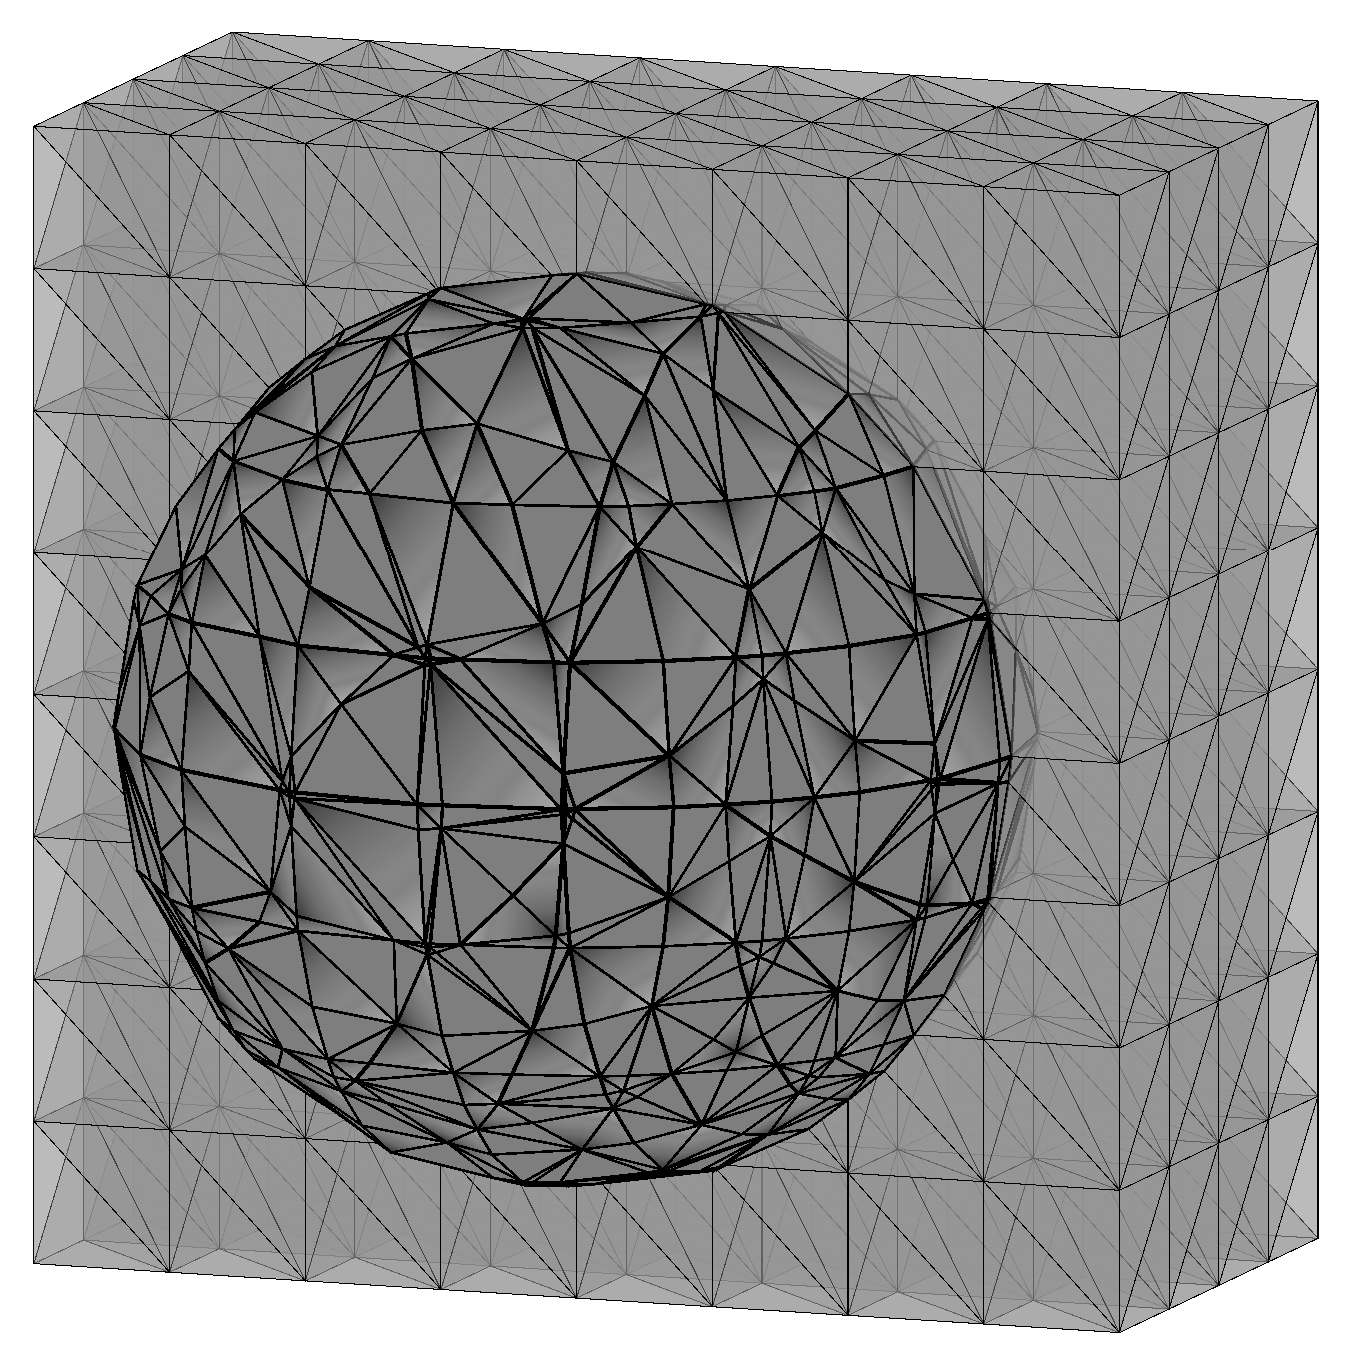
\includegraphics[width=0.51\textwidth]{trace_cutaway}
%\includegraphics[width=0.5\textwidth]{trace_mesh_blowup}}
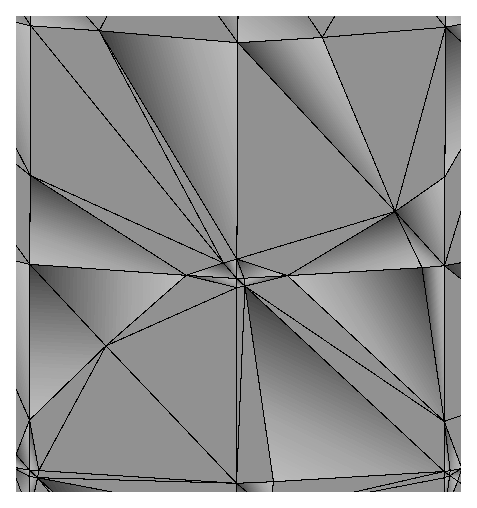
\includegraphics[width=0.46\textwidth]{trace_blowup}}
\caption{Bulk mesh cutaway with associated trace mesh (left); blowup of a trace mesh showing small and narrow elements (right).  
} \label{f:tracemeshes}
\end{figure}

This is the trace method and has two notable advantages:

\begin{itemize}
\item
{\it Only single mesh}: The main advantage is that both bulk and
interfacial effects can be computed using the same mesh.

\item
{\it Error estimates}: 
Optimal-order and regularity error estimates hold in the $H^1$ and $L_2$ norms.
\end{itemize}

\noindent
On a practical and theoretical levels the method exhibits three main challenges:

\begin{itemize}
\item
  {\it Implicit surface representation}: The simplest option of taking the distance function $d$ to define $\gamma$ and its Lagrange interpolant of $d_h$ to define $\Gamma$ is not generally practical as $d$ is rarely available in applications. It is generally more practical to assume that the discrete surface $\Gamma$ is derived from a more general level set representation $\phi$ of $\gamma$.   We provide a brief discussion of general level set representations below.  
\item
{\it Surface integration}: Computing the finite element system is more cumbersome than in standard parametric surface FEMs since both the mesh $\mathcal{F}$ and the finite element space $\V(\mathcal F)$ are derived from their corresponding bulk counterparts. These difficulties are manageable in the case of the piecewise linear method presented here, but become significantly more cumbersome when a higher-order surface approximation is used.
\item
{\it Linear algebra and stabilization}: In contrast to parametric surface FEMs there is no obvious practical basis for $\V(\mathcal F)$, only spanning sets derived from subsets of the bulk space $\V(\mathcal T)$.  In practice such a spanning set is derived from the degrees of freedom for $\V(\mathcal T)$ corresponding to elements touching $\Gamma$.  Degenerate modes arise from this procedure.  These are either handled at the linear algebra level or by various stabilization procedures.

\end{itemize}

Theoretical study of trace FEMs is also more involved than for parametric surface FEMs.   One prominent issue is that the surface mesh $\mathcal{F}$ does not consist of shape regular elements, as is documented in Figure \ref{f:tracemeshes}.  This is because the faces in $\mathcal{F}$ consist of {\it arbitrary} intersections of hyperplanes with simplices (planes and tetrahedra for $n=2$).  Thus elements may be arbitrarily small with respect to the bulk mesh-size $h$ or fail to satisfy a minimum angle condition, and it is not possible to directly employ standard error estimation techniques.  Properties of the ``high-quality'' bulk mesh $\T$ and finite element space $\V(\mathcal T)$ must be invoked instead, which in turn requires careful use of extensions and restrictions of functions to and from $\gamma$ and $\Gamma$.   For purposes of intuition, it is however useful to note that the surface mesh $\mathcal{F}$ does inherit some structure from the regularity of the bulk mesh $\T$.  Elements in $\mathcal{F}$ for example satisfy a maximum-angle condition \cite{ORX12}, and each element in $\mathcal{F}$ also shares a vertex with a shape-regular element of diameter equivalent to $h$ \cite{DO12}.

Below we prove a priori and a posteriori error estimates for a piecewise linear trace FEM.  In keeping with the previous section, we concentrate on surface representations and regularity in our discussion.  In particular, we only assume that $\gamma$ is $C^2$, whereas previous approaches require that $\gamma$ be $C^3$.  The recent article \cite{OR17} provides a broader survey of trace FEMs, including discussion of topics such as higher-order versions, stabilization procedures, and space-time trace FEMs that we omit here.  

%%%%%%%%%%%%%%%%%%%%%%%%%%%%%%%%%%%%%%%%%%%%%%%%%%%%%%%%%%%%%%%%%%%%%%%%%%%%%%%%%
\subsection{Preliminaries}\label{S:trace-prelim}
%%%%%%%%%%%%%%%%%%%%%%%%%%%%%%%%%%%%%%%%%%%%%%%%%%%%%%%%%%%%%%%%%%%%%%%%%%%%%%%%%

%--------------------------------------------------------------------------------
{\bf Bulk and Surface Meshes.}
%--------------------------------------------------------------------------------
Below we need to carefully distinguish between mesh structures defined relative to the surface mesh $\mathcal{F}$ and those defined relative to the volume mesh $\T$.  First note that we shall consistently denote by $F$ ($n$-dimensional) surface elements lying in $\mathcal{F}$, which as we have noted above may not be shape-regular.  In addition, $T$ will be used to denote $(n+1)$-simplices lying in $\T$.  Given a face $F \in \mathcal{F}$, we denote by $T_F$ the simplex in which $F$ lies (or one of them if $F$ is a face shared by two bulk elements).  In addition, given $T \in \T$ we denote by $\omega_\T^1(T)$ the patch of elements of $\T$ surrounding $T$ (first ring)
%
\[
\omega_\T^1(T) := \bigcup \big\{T'\in\T: ~~ T'\cap T \neq \emptyset  \big\},
\]
%
and by $\omega_\T^2(T)$ the patch of elements of $\T$ surrounding $\omega_\T^1(T)$ (second ring). We also define 
%
$$h_F={\rm diam}(T_F) \quad F \in \mathcal{F},$$
%
whence the local mesh size of the face element $F$ is taken to be the diameter of the corresponding bulk element.   Note that it is possible that ${\rm diam}(F) << h_F.$  We will also denote by $h_T$ the diameter of elements $T\in\T$. We finally let
%
$$\T_\Gamma := \big\{T \in \T: ~~ \Gamma \cap T \neq \emptyset \hbox{ or } \gamma \cap T \neq \emptyset \big\}$$
%
be the set of elements of $\T$ touching either $\Gamma$ or $\gamma$.  

\medskip\noindent
%--------------------------------------------------------------------------------
{\bf Geometric Assumptions.}  %\label{sec:trace_geo}
%--------------------------------------------------------------------------------
Above we described $\Gamma$ as the zero level set of an approximate distance function $d_h$.  In this section we first place abstract requirements on $\Gamma$ that are sufficient to obtain optimal-order and regularity a priori error estimates and then prove that these requirements are satisfied on sufficiently fine bulk meshes $\T$ when $\Gamma$ is built from a suitably general level set description of $\gamma$.   We now list three main geometric assumptions.

\begin{itemize} 
\item {\bf Description of $\Gamma$.}  We assume that $\Gamma$ is a polyhedral surface whose faces $F\in\mathcal{F}$ consist of the intersection of hyperplanes with simplices $T\in\T$. We further assume that $\Gamma \subset \mathcal{N}$ with $\mathcal{N}$ the tubular neighborhood defined in \eqref{N:def}.
\item {\bf Geometric resolution of $\gamma$.}  Let $d$ be the distance function to $\gamma$, $\bnu = \nabla d$ and $\bnu_\Gamma$ be the outward unit normal on $\Gamma$.  We assume that
\begin{align}
\label{trace:geo_res_assumption}
\|d\|_{L_\infty(F)} + h_F \|\bnu-\bnu_\Gamma\|_{L_\infty(F)}
\lesssim h_F^2 |d|_{W^2_\infty(\mathcal{N})}
\quad F \in \mathcal{F}.
\end{align}
This assumption is sufficient to ensure optimal decay of the geometric consistency error in a priori error estimates.  
\item {\bf Local flattening.}  We assume that for each $T \in \T$ with $T \cap \gamma \neq \emptyset$, there is a ball $B_R$ of radius $R$ with $R \simeq 1$ (independent of $h_T$) such that $T \subset B_{R/2}$ and there is a uniformly bi-$C^2$ map
\begin{align}
\label{ass:flattening}
\Phi:B_R \rightarrow \mathbb{R}^3, \quad \Phi(\gamma \cap B_R) \hbox{ lies in a hyperplane.}
\end{align}
\end{itemize} 

The flattening assumption \eqref{ass:flattening} follows from the $C^2$ nature of the surface $\gamma$ provided elements $T\in\T$ intersecting $\gamma$ are sufficiently fine with respect to the inverse of the maximum principal curvature. The flattening map $\Phi$ may be constructed by expressing $\gamma$ as a $C^2$ graph over tangent hyperplanes of $\gamma$, with the radius of the domain of these graphs bounded by the inverse of the maximum principal curvature of $\gamma$ (cf. \cite[Appendix C]{Ev98} for the construction of $\Phi$; the bound for $R$ follows from the definition of curvature).

\medskip\noindent
%--------------------------------------------------------------------------------
{\bf Level set representations.}
%--------------------------------------------------------------------------------
While we prove our results below under the abstract geometric resolution assumption \eqref{trace:geo_res_assumption} involving the distance function, in practice trace methods often build the discrete surface $\Gamma$ from a more general implicit representation of $\gamma$.   Such a representation may be obtained by assuming that $\gamma$ is the zero level set of a {\it level-set function} $\phi:\mathcal{N} \rightarrow \mathbb{R}$
%
$$\gamma=\{\bx \in \mathcal{N}: ~~ \phi(\bx)=0\}.$$
%
Broadening our assumptions concerning implicit representation of $\gamma$ is important in many practical applications.  Because the distance function $d$ has a closed form expression only if $\gamma$ is a sphere or a torus, there are many settings where $\gamma$ may easily be represented as a level set even if $d$ is not available. A simple example is the ellipsoid given by $\gamma=\left \{\bx \in \mathbb{R}^3: \frac{x^2}{a^2}+\frac{y^2}{b^2}+\frac{z^2}{c^2}-1=0 \right \}$.  {\it Level set methods} in which an evolving free boundary is computationally approximated by the level set of a discrete function are also popular in many applications.  In this case it is also natural to define $\gamma$ via a generic level set function $\phi$ rather than restrict attention to the distance function $d$.  

Our essential assumptions concerning $\phi$ are that $\phi \in C^2(\mathcal{N})$ and 
\begin{align}
\label{eq:phi_assumption}
\nabla \phi(\bx) \cdot \bnu(\bx) \ge c_\phi >0 \quad \forall \bx \in \gamma.
\end{align}
Because $\gamma$ is a level set of $\phi$, $|\nabla \phi|=|\nabla \phi \cdot \nu|$ on $\gamma$, so the assumption \eqref{eq:phi_assumption} is equivalent to assuming that $\nabla \phi$ is nondegenerate on $\gamma$ and points in the same direction as $\bnu=\nabla d$. Let $\phi_h \in \V(\mathcal T)$ be an approximation to $\phi$ satisfying 
%
\begin{align}
\label{eq:phih_assumption}
\|\phi-\phi_h\|_{L_\infty(T)} + h_T\|\phi-\phi_h\|_{W_\infty^1(T)}
  \lesssim h_T^2 \|\phi\|_{W^2_\infty(\mathcal{N})}
\quad T \in \T, 
\end{align}
%
and define the discrete surface $\Gamma$ by 
%
$$\Gamma : = \big\{\bx \in \mathcal{N}: ~~ \phi_h(\bx)=0 \big\}.$$

\begin{lemma}[geometric resolution]\label{L:geo-res}
Let $\gamma$ be $C^2$. Under the above assumptions, the inequality \eqref{trace:geo_res_assumption} holds for $h:=\max_{T \in \T} h_T$ sufficiently small, namely
\begin{align}
\label{eq:phi_properties}
\|d\|_{L_\infty(F)}+ h_F \|\bnu-\bnu_\Gamma\|_{L_\infty(F)}
  \lesssim h_F^2 \|\phi\|_{W^2_\infty(\mathcal{N})}
\quad F \in \mathcal{F}.
\end{align}
\end{lemma}
\begin{proof}

First let $\bx \in \mathcal{N}$, for which the projection $\bP_d(\bx)$ on $\gamma$ is uniquely defined. Let $\zeta(s) := \nabla \phi\big( s\bx + (1-s) \bP_d(\bx) \big)\cdot\bnu(\bx)$ and compute
$$
\begin{aligned}
|(\nabla \phi \cdot \bnu) (\bx) &- (\nabla \phi \cdot \bnu) (\bP_d(\bx) )| =
|\zeta(1)-\zeta(0)| = \left |\int_0^1 \zeta'(s) ds \right |
\\
&= \left | \int_0^1 \nabla \big(\nabla\phi\big( s\bx + (1-s) \bP_d(\bx) \big)\cdot\bnu(\bx) \big) \cdot \big(\bx-\bP_p(\bx) \big) \right |
\\ & \le  |\bx- \bP_d(\bx)| \, \|\nabla (\nabla \phi \cdot \nu)\|_{L_\infty([\bP_d(x), \bx])}.
\end{aligned}
$$
%
Since $(\nabla \phi \cdot \bnu) (\bP_d(\bx)) \ge c_\phi>0$, $\phi \in C^2(\mathcal{N})$, and $\bnu \in C^1(\mathcal{N})$, there thus exists a constant $C_\phi\le\frac{1}{2K_\infty}$ (depending on $\|\phi\|_{W_\infty^2(\mathcal{N})}$ and $|d|_{W_\infty^2(\mathcal{N})}$) such that
%
\[
(\nabla \phi \cdot \bnu)(\bx) \ge \frac{c_\phi}{2}
\quad \forall \,\bx \in \mathcal{N}_{\phi}:=\big\{\by\in\Omega: ~ |d(\by)|\le C_\phi  \big\} \subset \mathcal{N},
\]
%
according to \eqref{N:def}. Therefore, for any $\bx \in \mathcal{N}_\phi$ we have $\phi(\bP_d(\bx))=0$ and
%
$$
|\phi(\bx)| = \left | \int_0^1 \nabla \phi(s\bx+(1-s)\bP_d(\bx)) \cdot (\bx-\bP_d(\bx)) \right | \simeq |\bx - \bP_d(\bx)| = |d(\bx)|,
$$
%
because $\bx-\bP_d(\bx) = |\bx-\bP_d(\bx)| \bnu(\bx)$. Given any face $F \in \mathcal{F}$ of $\Gamma$, we realize that $\phi_h(\bx)=0$ for all $\bx\in F$ and
%
\[
|\phi(\bx)| = |\phi(\bx)-\phi_h(\bx)| \lesssim h_F^2 \|\phi\|_{W^2_\infty(\mathcal{N})}.
\]
%
If $h\ge h_F$ is sufficiently small, then $\bx\in\mathcal{N}_\phi$ and $|d(\bx)| \simeq |\phi(\bx)| \lesssim h_F^2|\phi|_{W^2_\infty(\mathcal{N})}$. This is the desired bound for the first term on the left hand side of \eqref{eq:phi_properties}.

  
To prove the remaining bound in \eqref{eq:phi_properties}, we note that for $\bx \in F \in \mathcal{F}$, we have $\bnu_\Gamma(\bx)= \frac{ \nabla \phi_h(\bx)}{|\nabla \phi_h(\bx)|}$ and $\bnu(\bx) = \nu(\bP_d(\bx)) = \frac{\nabla \phi(\bP_d(\bx))}{|\nabla \phi (\bP_d(\bx))|}$. Consequently, for such $\bx \in \Gamma$, we use \eqref{eq:phih_assumption}, the bound $|d(\bx)| \lesssim h_F^2$ already proved, and the $C^2$ nature of $\phi$ to obtain
\begin{align*}
\begin{aligned}
\left |(\bnu_\Gamma-\bnu)(\bx) \right| &= \left |\frac{ \nabla \phi_h(\bx)}{| \nabla \phi_h(\bx)|}-\frac{\nabla \phi(\bP_d(\bx))}{|\nabla \phi (\bP_d(\bx))|} \right| 
\\ & \le \left |\frac{ \nabla \phi_h(\bx)}{|\nabla \phi_h(\bx)|}-\frac{ \nabla \phi(\bx)}{|\nabla \phi(\bx)|} \right | + \left | \frac{ \nabla \phi(\bx)}{|\nabla \phi(\bx)|}-\frac{\nabla \phi(\bP_d(\bx))}{|\nabla \phi (\bP_d(\bx))|}\right | \\ & \lesssim \big(h_F + h_F^2\big) \|\phi\|_{W^2_\infty(\mathcal{N})} \lesssim h_F \|\phi\|_{W^2_\infty(\mathcal{N})}.
\end{aligned}
\end{align*}  
This completes the proof.
\end{proof}
 
Thus we have shown that it is possible to define the discrete surface $\Gamma$ using a generic level set representation of $\gamma$ in such a way that $\Gamma$ has the same geometric approximation properties as if it were derived more directly from the distance function $d$.  Below we assume practical access to the distance function $d$ and associated geometric properties (curvatures and normal vectors) in two further places: the first one is the definition of the right hand side $F_\Gamma$ in formulating the trace FEM and the second one is the definition of geometric a posteriori error estimators.  As outlined in \cite{DemlowDziuk:07}, it is computationally feasible to accurately approximate $d(\bx)$, $\bP_d(x)$, and $\nu(\bx)$ for $\bx \in \Gamma$ under the assumption that we have access to a level set function $\phi$ with the properties assumed above.  In outline, the foundational building block of this procedure is a numerical approximation to $\bP_d(\bx)$.  Two such algorithms are proposed in \cite{DemlowDziuk:07}, one being Newton's method and the other an ad hoc first order method; cf. \cite{Gr17} for generalizations and analysis of these methods.  Once $\bP_d(\bx)$ is computed, we then have
%
\[
|d(\bx)| = |\bx - \bP_d(\bx)|,
\quad
\nu(\bx)= \frac{\nabla \phi(\bP_d(\bx))}{|\nabla \phi(\bP_d(\bx))|},
\quad\bW(\bP_d(\bx))= \nabla \frac{\nabla \phi(\bP_d(\bx))}{|\nabla \phi(\bP_d(\bx))|}.
\]
%
These relationships allow for the computation of all geometric information required to bound geometric errors in the trace method a posteriori.  In addition, because we may reasonably assume access to $\bP_d$ it is in turn reasonable to assume a consistent definition of the right hand side $F_\Gamma$, that is, $F_\Gamma = \frac{q}{q_\Gamma} f \circ \bP_d$.  A different definition of $F_\Gamma$ would lead to an additional consistency term in the results below.
  
  
\medskip\noindent
%--------------------------------------------------------------------------------
{\bf Harmonic Extension and Traces.}
%--------------------------------------------------------------------------------
Here we collect instrumental results for our proofs of a priori and a posteriori error estimates. For the latter we use the fractional-order space $H^{3/2}(\Omega)$, so we first define the seminorm of $H^{1+s}(\Omega)$
%
  $$|\tv|_{H^{1+s}(\Omega)}^2 := \sum_{|\alpha|=1} \iint_{\Omega \times \Omega} \frac{|D^\alpha \tv(x)-D^\alpha \tv(y)|^2}{|x-y|^{n+2s}} \hspace{1pt} {\rm d}x \hspace{1pt}{\rm d}y$$
%
for a Lipschitz domain $\Omega\subset\mathbb{R}^n$ and $0<s<1$, and corresponding norm
$$\|\tv\|_{H^{1+s}(\Omega)}^2 =\|\tv\|_{H^1(\Omega)}^2 + |\tv|_{H^{1+s}(\Omega)}^2.$$

Our first lemma is a standard extension result which may for example be found in \cite[Theorem 1.4.3.1]{G85}.  

\begin{lemma}[$H^{1+s}$ extension]
\label{lem:standard_extension}
Let $D$ be a bounded Lipschitz domain in $\mathbb{R}^n$, $n\ge2$.  Then there is an extension operator $E: H^{1+s}(D) \rightarrow H^{1+s}(\mathbb{R}^n)$ such that 
\begin{align}
\label{extension}
\|E\tv\|_{H^{1+s}(\mathbb{R}^n)} \lesssim \|\tv\|_{H^{1+s}(D)} \quad \forall \,s\in [0,1), \quad \forall \tv \in H^{1+s}(D).
\end{align}
\end{lemma}

We also state a trace result relating $H^1(\mathbb{R}^2)$ and $H^{3/2}(\mathbb{R}^3)$; this is a special case of \cite[Theorem 7.58]{Ad75}.   
\begin{lemma}[trace]
\label{lem:special_trace}
If $\tv \in H^{3/2}(\mathbb{R}^n)$, $n\ge2$, and $\mathbb{P}$ is any $(n-1)$-dimensional hyperplane in $\mathbb{R}^n$, then
\begin{align}
\label{special_trace}
\|\tv\|_{H^1(\mathbb{P})}  \lesssim \|\tv\|_{H^{3/2}(\mathbb{R}^n)}.
\end{align}
\end{lemma}

The following is an important technical lemma which expresses traces relationships between norms on surface elements (flat or curved) and corresponding norms on bulk elements.  An essential component of these estimates is that they allow for surfaces to cut through bulk elements in an arbitrary fashion.   Such estimates were essential in the proof of the first a posteriori estimates for trace methods in \cite{DO12}.  In the context of a priori error estimates for trace methods, these provide a substantially simplified proof of error bounds when compared with the original proofs given in \cite{ORG09}; cf. \cite{HH02, HH04, BHL15, Re15}.  


\begin{lemma}[trace estimates for cut elements]
\label{L:trace-est}
Let $D\subset \mathbb{R}^n$ ($n \ge 2$) be a (not necessarily bounded) Lipschitz domain, and let $D_{n-1}$ be the intersection of $D$ with an arbitrary hyperplane of dimension $n-1$.  Then
\begin{align}
\label{general_trace_est}
\|\tv \|_{L_2(D_{n-1})} \lesssim \|\tv\|_{H^1(D)} \quad \forall \tv \in H^1(D),
\end{align}
where the hidden constant depends on the Lipschitz nature of $D$ but not on the orientation or size of $D_{n-1}$.  In particular, let $F \in \mathcal{F}$ with $F \subset T \in \T$. Then
\begin{align}
\label{trace_est}
\|\tv\|_{L_2(F)} \lesssim h_T^{-1/2} \|\tv\|_{L_2(T)} + h_T^{1/2}\|\nabla \tv \|_{L_2(T)}
\quad \forall \tv \in H^1(T).
\end{align}
In addition, given $T \in \T$ there hold
\begin{align}
\label{curved_trace_est} 
\|\tv\|_{L_2(T \cap \gamma)} \lesssim h_T^{-1/2} \|\tv\|_{L_2(T)}+ h_T^{1/2} \|\nabla \tv\|_{L_2(T)} \quad \forall \tv \in H^1(T),
\end{align}
and
\begin{align}
\begin{aligned}
\label{H32_curved_trace}
h_T^{-1} & \|\tv\|_{L_2(T \cap \gamma)}  + \|\nabla_\gamma \tv\|_{L_2(T \cap \gamma)} 
\\ & \lesssim h_T^{-3/2} \|\tv\|_{L_2(T)} + h_T^{-1/2} \|\nabla \tv\|_{L_2(T)} + |\tv|_{H^{3/2}(T)} \quad\forall \tv \in H^{3/2}(T).
\end{aligned}
\end{align}
\end{lemma}

\begin{proof}
The estimate $\eqref{general_trace_est}$ is a special case of \cite[Lemma 5.19]{Ad75}.  The scaled result \eqref{trace_est} follows by a standard scaling argument.  

To prove \eqref{curved_trace_est} and \eqref{H32_curved_trace} we employ a flattening argument.  First let $\hat{K}$ be the unit reference simplex in $\mathbb{R}^n$ with standard affine reference mapping $\varphi: \hat{K} \rightarrow T$ satisfying $\|\nabla \varphi\|_{L_\infty(\hat K)} \lesssim h_T$ and $\|(\nabla \varphi)^{-1}\|_{L_\infty(T)} \lesssim h_T^{-1}$.  Let now $\Phi$ be the flattening map in assumption \eqref{ass:flattening}.  It is possible to extend $\Phi$ to all of $\mathbb{R}^n$ so that the resulting extension is also $C^2$, still flattens $T \cap \gamma$, and has derivative bounded above and below away from 0.  To see this, take a smoothly weighted average of $\Phi$ and the identity with weight 1 for $\Phi$ on $B_{R/2}$ and weight 0 outside of $B_R$.  Having thus extended $\Phi$, we define $\widetilde\Phi:=\varphi^{-1} \circ \Phi \circ \varphi$.  It is easy to check that $\widetilde\Phi$ and $\widetilde\Phi^{-1}$ are uniformly bounded in $C^2$ and that $\widetilde\Phi(\varphi^{-1} (T \cap \gamma))$ lies in some $(n-1)$-dimensional hyperplane $\mathbb{P}$.

For $\tv \in H^1(T)$ with $T \in \mathcal T$ satisfying $|T\cap \gamma|>0$, let now $\widehat{\tv}=\tv \circ \varphi$. We first prove \eqref{H32_curved_trace} upon transforming to the reference element back and forth. We start with a simple scaling argument
%
\[
\frac{|\varphi^{-1}(T\cap\gamma)|}{|T\cap\gamma|} \approx h_T^{1-n},
\]
%
regardless of the actual size and orientation of $T\cap\gamma$ relative to $T\in\T$. Hence, applying a standard change of variables involving $\varphi$ yields
%
\[
h_T^{1-n} \Big( \|\tv\|_{L_2(T \cap \gamma)}^2  + h_T^2\|\nabla_\gamma \tv \|_{L_2(T \cap \gamma)}^2 \Big) \approx \|\widehat{\tv}\|_{H^1(\varphi^{-1}(T \cap \gamma))}^2.
\]
%
We next resort to the extension operator $E:H^{3/2}(\hat K)\to H^{3/2}(\mathbb{R}^n)$ in Lemma \ref{lem:standard_extension} ($H^{1+s}$ extension), the smoothness of $\widetilde\Phi^{-1}$, the fact that $\widetilde\Phi( \varphi^{-1}(T \cap \gamma))\subset\mathbb{P}$, the trace inequality \eqref{special_trace}, the smoothness of $\widetilde\Phi^{-1}$ again, and the boundedness \eqref{extension} of $E$ in $H^{3/2}(\hat K)$, in this order, to arrive at
%
\begin{align*}
\|\widehat{\tv}\|_{H^1(\varphi^{-1}(T \cap \gamma))} &=
\|E \widehat{\tv}\|_{H^1(\varphi^{-1} (T \cap \gamma))}
\\ & \lesssim \|E \widehat{\tv} \circ \widetilde\Phi^{-1}\|_{H^1\big(\widetilde\Phi( \varphi^{-1}(T \cap \gamma))\big)}
\\ & \lesssim \|E \widehat{\tv} \circ \widetilde\Phi^{-1}\|_{H^1(\mathbb{P})}
\\ & \lesssim \|E \widehat{\tv} \circ \widetilde\Phi^{-1}\|_{H^{3/2}(\mathbb{R}^n)}
\\ & \lesssim \|E \widehat{\tv}\|_{H^{3/2}(\mathbb{R}^n)}
\\ & \lesssim \|\widehat{\tv}\|_{H^{3/2}(\hat{K})}.
\end{align*}
%
The desired estimate \eqref{H32_curved_trace} finally follows from a scaling argument
from $\hat K$ to $T$ employing again the map $\varphi$:
%
\[
\|\widehat{\tv}\|_{H^{3/2}(\hat{K})}^2
\lesssim h_T^{-n} \Big(\|\tv\|_{L_2(T)}^2 + h_T^2 \|\nabla \tv\|_{L_2(T)}^2 + h_T^3 |\tv|_{H^{3/2}(T)}^2 \Big).
\]
%

To prove \eqref{curved_trace_est}, we argue similarly to above except that we now employ
$E:H^1(\hat K) \to H^1(\mathbb{R}^n)$ and \eqref{general_trace_est} instead of \eqref{special_trace}.  Doing so yields
$$\begin{aligned}
 h_T^{(1-n)/2} \|\tv\|_{L_2(T \cap \gamma)} & \lesssim \|\widehat{\tv}\|_{L_2(\varphi^{-1}(T \cap \gamma))}
\\ & = \|E \widehat{\tv}\|_{L_2(\varphi^{-1} (T \cap \gamma))}
\\ & \lesssim \|E \widehat{\tv} \circ \widetilde\Phi^{-1}\|_{L_2(\widetilde\Phi( \varphi^{-1}(T \cap \gamma)))}
\\ & \lesssim \|E \widehat{\tv} \circ \widetilde\Phi^{-1}\|_{L_2(\mathbb{P})}
\\ & \lesssim \|E \widehat{\tv} \circ \widetilde\Phi^{-1}\|_{H^1 (\mathbb{R}^n)}
\\ & \lesssim \|E \widehat{\tv}\|_{H^1(\mathbb{R}^n)}
\\ & \lesssim \|\widehat{\tv}\|_{H^1(\hat{K})}
\\ & \lesssim h_T^{-n/2} \|\tv\|_{L_2(T)} + h_T^{(2-n)/2} \|\nabla \tv\|_{L_2(T)}.
\end{aligned}$$
Multiplying both sides by $h_T^{(n-1)/2}$ gives the desired bound \eqref{curved_trace_est}.
\end{proof}

%%%%%%%%%%%%%%%%%%%%%%%%%%%%%%%%%%%%%%%%%%%%%%%%%%%%%%%%%%%%%%%%%%%%%%%%%%%%%
\subsection{A Priori Error Estimates}\label{S:trace-apriori}
%%%%%%%%%%%%%%%%%%%%%%%%%%%%%%%%%%%%%%%%%%%%%%%%%%%%%%%%%%%%%%%%%%%%%%%%%%%%%

We recall that we use the notation $ h := \max_{T \in \T} h_T$ and that we omit to mention the explicit dependence on the shape regularity constant of $\mathcal T$ in most estimates.

\medskip\noindent
%----------------------------------------------------------------------------
{\bf Geometric resolution and extensions.}  %\label{sec:apriori_geo_res_ass}
%----------------------------------------------------------------------------
%
Given a surface $\gamma$ of class $C^2$ and $\wu \in H^2(\gamma)$, 
Proposition \ref{P:H2-extension} ($H^2$ extension) yields the existence of an extension $u$ of $\wu$ to a tubular neighborhood $\mathcal{N}(\delta)$ with $\delta$ sufficiently small with respect to $\frac{1}{2 K_\infty}$ lying in $H^2(\mathcal{N(\delta)})$ and satisfying
\begin{align}
\label{H2extend}
\|u\|_{H^2(\mathcal{N}(\delta))} \lesssim \delta^{1/2} |d|_{W_\infty^2(\mathcal{N})}\|\wu\|_{H^2(\gamma)}.
\end{align}

\begin{itemize}
\item {\bf First assumption on geometric resolution by the bulk mesh.} We assume
%
\begin{equation}\label{e:TGamma}
\bigcup \big\{\omega_\T^1(T): ~ T \in \T_{\Gamma}\big\} \subset \mathcal{N}(\delta)
\end{equation}
%
with $\delta \simeq h$ sufficiently small so that \eqref{H2extend} holds.
%
\item {\bf Second assumption on geometric resolution by the bulk mesh.} We assume that the layer $D_{\Gamma, \gamma}:=\{s\bx + (1-s) \bP_d(\bx): \, \bx \in \Gamma \hbox{ and } 0 \le s \le 1\}$ satisfies 
\begin{align}
\label{ass:skinlayer}
D_{\Gamma, \gamma} \subset \bigcup \big\{T: ~T\in\T_\Gamma\big\}.
\end{align}
%
This clearly holds for $h$ sufficiently small because the Hausdorff distance between $\gamma$ and $\Gamma$ satisfies $\dist_H(\gamma,\Gamma)\lesssim h^2$ according to \eqref{trace:geo_res_assumption}.

\item
{\bf Uniform Poincar\'e-Friedrichs estimate on $\Gamma$.} We assume that
%
\begin{align} \label{trace-poin-unif}
\|\tv\|_{L_2(\Gamma)} \lesssim \|\nabla \tv\|_{L_2(\Gamma)}
\quad\forall \tv \in H^1_\#(\Gamma)
\end{align}
%
holds with uniform constant. According to the discussion below \eqref{poin-unif} (uniform Poincar\'e-Friedrichs constant), this only requires that $\Gamma \subset \mathcal{N}(1/2K_\infty)$ and that $\bnu\cdot \bnu_\Gamma \ge c >0$ on $\Gamma$. These conditions are easily checkable and valid asymptotically.
%
\end{itemize}

\medskip\noindent
%------------------------------------------------------------------------------
{\bf Approximation properties of trace finite element space.}
%------------------------------------------------------------------------------
%
We next state a fundamental approximation bound for the trace FEM, which we prove under the regularity assumption that $\gamma$ is of class $C^2$. We emphasize that this assumption is less restrictive than the hypotheses of previous approximation bounds for trace estimates, which assume that $\gamma$ is of class $C^3$.  

\begin{lemma}[trace approximation]
\label{lem:trace_approx}
Let $\gamma$ be of class $C^2$ and the geometric resolution assumptions \eqref{trace:geo_res_assumption}, \eqref{ass:flattening}, \eqref{e:TGamma}, and \eqref{ass:skinlayer} hold.  Then
%
\begin{equation}\label{e:trace_approx}
  \inf_{\tV \in \V(\mathcal F)} \|\nabla_\Gamma (\wu\circ\bP_d-V)\|_{L_2(\Gamma)}
  \lesssim h\|\wu\|_{H^2(\gamma)}.
  \end{equation}
\end{lemma}
\begin{proof}
Let $\delta \simeq h$ be sufficiently small so that \eqref{e:TGamma} is valid.
Let $\interp^{\textrm{sz}}$ be the standard Scott-Zhang interpolation operator on $\T$, and take $V=\interp^{\textrm{sz}} u$ with $u\in H^2(\Nd)$ given by Proposition \ref{P:H2-extension} ($H^2$ extension) and satisfying \eqref{H2extend}. We then denote $u_d=\wu\circ\bP_d, V_d=V\circ\bP_d$, add and subtract multiple terms, and apply the triangle inequality to find that
%
\[
\| \nabla_\Gamma(u_d-V)\|_{L_2(\Gamma)}  \lesssim  \sum_{i=1}^7 I_i
\]
%
where
%
\begin{align*}
I_1 &:= \|\nabla_\Gamma(u_d-V_d)\|_{L_2(\Gamma)},
\\ I_2 &:=   \|\Pi_\Gamma [\nabla V_d-(\nabla V) \circ \bP_d]\|_{L_2(\Gamma)} ,
\\ I_3 &:= \|\Pi_\Gamma [\nabla V\circ \bP_d - \nabla u \circ \bP_d]\|_{L_2(\Gamma)} ,
\\ I_4 &:= \|\Pi_\Gamma [\nabla u \circ \bP_d - (\interp^{\textrm{sz}} \nabla u) \circ \bP_d]\|_{L_2(\Gamma)},
\\ I_5 &:= \|\Pi_\Gamma [(\interp^{\textrm{sz}} \nabla u) \circ \bP_d - \interp^{\textrm{sz}} \nabla u] \|_{L_2(\Gamma)} ,
\\ I_6 &:= \|\Pi_\Gamma [\interp^{\textrm{sz}} \nabla u - \nabla u]\|_{L_2(\Gamma)},
\\ I_7 &:= \|\Pi_\Gamma [ \nabla u -\nabla V]\|_{L_2(\Gamma)}.
\end{align*}
%
Here we have applied the interpolation operator $\interp^{\textrm{sz}}$ componentwise to the $(n+1)$-vector $\nabla u$ and used that $\nabla_\Gamma = \Pi_\Gamma \nabla$. We next estimate each term separately.

In order to bound terms $I_1$ and $I_3$, we employ Lemma \ref{L:norm-equiv} (norm equivalence) between $\gamma$ and $\Gamma$ and recall that $|\nabla_\gamma \tv| \le |\nabla \tv|$ pointwise to find that
%
\begin{align*}
  I_1+I_3 \lesssim \Big (\sum_{T \in \T_\Gamma} \|\nabla (u-V)\|_{L_2(T \cap \gamma)} ^2 \Big)^{1/2}.
\end{align*}  
%
We next apply the trace estimate \eqref{curved_trace_est}, utilize standard approximation properties of $\interp^{\textrm{sz}}$, and finally use the bound \eqref{H2extend} to obtain
%
\begin{align*}
I_1+I_3 & \lesssim \Big(\sum_{T\in \T_\Gamma} h_T^{-1} \|\nabla (u-V)\|_{L_2(T)}^2 + h_T\|D^2 u\|_{L_2(T)}^2 \Big)^{1/2}
\\ & \lesssim h^{1/2} \|u\|_{H^2(\mathcal{N}(\delta))} \lesssim h \|\wu\|_{H^2(\gamma)}.
\end{align*}
%
Here we have used that $\nabla \nabla V=0$ elementwise since $V$ is piecewise linear. Similar arguments lead to the following estimate for $I_4$
%
\[
I_4 \lesssim \Big(\sum_{T\in \T_\Gamma} h_T^{-1} \|\nabla u-\interp^{\textrm{sz}} \nabla u\|_{L_2(T)}^2 + h_T\|\nabla(\nabla u-\interp^{\textrm{sz}} \nabla u)\|_{L_2(T)}^2 \Big)^{1/2},
\]
%
as well as $I_4 \lesssim h \|\wu\|_{H^2(\gamma)}$ provided $\|\nabla \interp^{\textrm{sz}} \nabla u\|_{L_2(T)} \lesssim \|D^2 u\|_{L_2(\omega_\T^1(T))}$. To show this estimate we let $\overline{\nabla u}_T := |\omega_\T^1(T)|^{-1} \int_{\omega_\T^1(T)} \nabla u$ be the meanvalue of $\nabla u$ in $\omega_\T^1(T)$ and exploit the stability of $\interp^{\textrm{sz}}$ in $H^1(T)$
%
\begin{align*}
  \|\nabla \interp^{\textrm{sz}} \nabla u\|_{L_2(T)}
  &= \|\nabla \interp^{\textrm{sz}} [\nabla u - \overline{\nabla u}_T]\|_{L_2(T)}
  \lesssim h_T^{-1} \|\interp^{\textrm{sz}}[\nabla u - \overline{\nabla u}_T]\|_{L_2(T)}
  \\ &
  \lesssim h_T^{-1} \|\nabla u - \overline{\nabla u}_T\|_{L_2(\omega_\T^1(T))}
  \lesssim \|D^2 u \|_{L_2(\omega_\T^1(T))}.
\end{align*}
%
Moreover, applying the trace estimate \eqref{trace_est} directly to the terms $I_6$ and
$I_7$ yields
%
\begin{align*}
I_6 & \lesssim \Big(\sum_{F \in \mathcal{F}} \|\interp^{\textrm{sz}} \nabla u-\nabla u\|_{L_2(F)}^2 \Big)^{1/2} 
\\ & \lesssim \Big(\sum_{T \in \T_\Gamma} h_T^{-1} \|\interp^{\textrm{sz}} \nabla u -\nabla u\|_{L_2(T)}^2 + h_T \|\nabla[\interp^{\textrm{sz}} \nabla u -\nabla u]\|_{L_2(T)}^2 \Big)^{1/2}
\lesssim h \|\wu\|_{H^2(\gamma)},
\end{align*}
%
and
\begin{align*}
I_7 & \lesssim \Big(\sum_{F \in \mathcal{F}} \|\nabla(u-V)\|_{L_2(F)}\Big)^{1/2}
\\ &
\lesssim \Big(\sum_{T \in \T_\Gamma} h_T^{-1} \|\nabla (u-V)\|_{L_2(T)}^2 + h_T \|D^2 u\|_{L_2(T)}^2\Big)^{1/2}
\lesssim h \|\wu\|_{H^2(\gamma)}. 
\end{align*}

In order to bound term $I_2$, we first note that
%
\[
\Pi_\Gamma [\nabla V_d-(\nabla V) \circ \bP_d] = \Pi_\Gamma (\Pi-d D^2d-\bI) (\nabla V) \circ \bP_d.
\]
%
An easy computation using the assumption \eqref{trace:geo_res_assumption} yields
%
$$|\Pi_\Gamma(\Pi-d D^2d - \bI)|  \lesssim |\Pi_\Gamma \Pi-\Pi_\Gamma| + |d| =|(\bnu \cdot \bnu_\Gamma) \bnu_\Gamma \otimes \bnu -\bnu \otimes \bnu|+ h^2 \lesssim h.$$
%
Thus employing the equivalence of norms on $\gamma$ and $\Gamma$, the trace estimate \eqref{curved_trace_est}, the $H^1$ boundedness of $\interp^{\textrm{sz}}$, and the boundedness \eqref{H2extend} of the extension yields
$$
\begin{aligned}
I_2 & \lesssim h \|\nabla \tV \circ \bP_d\|_{L_2(\Gamma)} \lesssim h \|\nabla V\|_{L_2(\gamma)} 
\\& \lesssim h^{1/2} \|\nabla V\|_{L_2(\T_\Gamma)} 
 \lesssim h^{1/2} \|u\|_{H^1(\mathcal{N}(\delta))}
 \lesssim h \|\widetilde u\|_{H^2(\gamma)}.
\end{aligned}
$$
We finally bound term $I_5$.  Given $\bx=\bP_d(\bx) + d(\bx)\nabla d(\bP_d(\bx)) \in \Gamma$, we infer that
%
\[
|\interp^{\textrm{sz}} \nabla u(\bx)-\interp^{\textrm{sz}} \nabla u(\bP_d(\bx))| \le \int_0^{d(\bx)} \Big| \nabla \big[\interp^{\textrm{sz}} \nabla u\big( \bP_d(\bx)+s\nabla d(\bP_d(\bx))  \big) \big] \Big| ds
\]
%
and $|d(\bx)|\lesssim h^2$ according to \eqref{trace:geo_res_assumption}, whence 
\[
I_5^2 \lesssim h^2 \int_\Gamma \int_0^{d(\bx)} \Big| \nabla \big[\interp^{\textrm{sz}} \nabla u\big( \bP_d(\bx)+s\nabla d(\bP_d(\bx))  \big) \big]\Big|^2 ds d\sigma(\bx) \lesssim h^2 \int_{D_{\Gamma,\gamma}} |\nabla \interp^{\textrm{sz}} \nabla u|^2.
\]
%
In view of assumptions \eqref{ass:skinlayer} and \eqref{e:TGamma}, and the
bound $\|\nabla \interp^{\textrm{sz}}\nabla u\|_{L_2(T)} \lesssim \|D^2 u\|_{L_2(\omega_\T^1(T))}$, we deduce
%
\[
I_5^2 \lesssim h^2 \|D^2 u\|_{L_2(\Nd)}^2 \lesssim h^3 \|D^2 \wu\|_{H^2(\gamma)}^2,
\]
%
and conclude the proof.
\end{proof}
  

\begin{theorem}[a-priori error estimates]
Let $\gamma$ be of class $C^2$ and let $\Gamma$ be so that the geometric assumptions \eqref{trace:geo_res_assumption}, \eqref{ass:flattening}, \eqref{e:TGamma}, \eqref{ass:skinlayer}, and \eqref{trace-poin-unif} are satisfied. Let $\wf\in L_{2,\#}(\gamma)$ and $\wu\in H^2(\gamma)$ solve \eqref{e:weak_relax}. If $U \in \V_\#(\mathcal F)$ is the finite element solution of \eqref{def:trace_fem} with $F_\Gamma =\frac{q}{q_\Gamma} \wf \circ \bP_d $, then
%
$$
\|\wu\circ\bP_d-U \|_{L_2(\Gamma)} + h \|\nabla_\Gamma (\wu\circ\bP_d-U)\|_{L_2(\Gamma)} \lesssim h^2 \|\wf\|_{L_2(\gamma)}.
$$
\end{theorem}

\begin{proof}
With the geometric resolution estimate~\eqref{trace:geo_res_assumption} and Lemma \ref{lem:trace_approx} (trace approximation) in hand, the proof is nearly identical to those of Theorem \ref{t:H1error} ($H^1$ a-priori error estimate) and Theorem \ref{t:L2_apriori} ($L^2$ a-priori error estimate) for parametric surface FEM. We thus sketch the proof without details.

\medskip\noindent
{\it Step 1: $H^1$ error estimate.}
Let $V \in\V(\mathcal F)$ achieve the infimum in \eqref{e:trace_approx}, $W:=V-U$, $u=\wu\circ\bP_d$, and write the error representation formula as
%
\[
\|\nabla_\Gamma (V-U)\|_{L_2(\Gamma)}^2 = \int_\Gamma \nabla_\Gamma u\cdot\bE_\Gamma \nabla_\Gamma W + \int_\Gamma \nabla_\Gamma (V-u)\cdot\nabla_\Gamma W,
\]
%
because $F_\Gamma = \frac{q}{q_\Gamma} \wf \circ \bP_d$.
In view of Lemma \ref{L:geom_consist_dist} (geometric consistency) and the geometric resolution estimate~\eqref{trace:geo_res_assumption} we deduce $|\bE_\Gamma| \lesssim h^2 |d|_{W^2_\infty(\mathcal{N})}$ and
%
\[
\Big| \int_\Gamma \nabla_\Gamma u\cdot\bE_\Gamma \nabla_\Gamma W  \Big|
\lesssim h^2 |d|_{W^2_\infty(\mathcal{N})} \|\wu\|_{H^1(\gamma)} \|\nabla_\Gamma W\|_{L_2(\Gamma)} \lesssim h \|\widetilde f\|_{L_2(\gamma)} \|\nabla_\Gamma W\|_{L_2(\Gamma)}.
\]
%
On the other hand, Lemma \ref{lem:trace_approx} (trace approximation) yields
%
\[
\Big|  \int_\Gamma \nabla_\Gamma (V-u)\cdot\nabla_\Gamma W \Big|
\lesssim h \|\wu\|_{H^2(\gamma)} \|\nabla_\Gamma W\|_{L_2(\Gamma)}.
\]
%  
The desired estimate follows from Lemma \ref{L:regularity} (regularity).

\medskip\noindent
{\it Step 2: $L_2$ error estimate.} Let $\bP_d^{-1}$ denotes the inverse of $\bP_d$ restricted to $\Gamma$. 
Let $\widetilde U:=U\circ\bP_d^{-1}:\gamma\to\mathbb{R}$ and
$\widetilde U_\# := \frac{q_\Gamma}{q}\widetilde U \in H^1_\#(\gamma)$; likewise,
let $u_\# := \frac{q}{q_\Gamma} u \in H^1_\#(\Gamma)$. We now solve dual problems on $\gamma$
%
\[
\wz\in H^1_\#(\gamma): \quad
\int_\gamma \nabla_\gamma \wz \cdot \nabla_\gamma w = \int_\gamma (\wu - \wU_\#) w
\quad \forall \, w\in H^1_\#(\gamma)
\]
%
and on $\Gamma$
%
\[
Z\in\V_\#(\mathcal F): \quad
\int_\Gamma \nabla_\Gamma Z \cdot \nabla_\Gamma W = \int_\Gamma (u_\#-U)W
\quad\forall \, W\in\V_\#(\mathcal F).
\]
%
Note that the right-hand sides $u_\#-U = \frac{q}{q_\Gamma}(\wu - \wU_\#)\circ\bP_d$ are compatible and Step 1 applies.
We set $\widetilde Z = Z \circ \bP_d$ and proceed as in Theorem \ref{t:L2_apriori} ($L_2$ a-priori error estimate) to deduce the error representation
%
\[
\|\wu-\wU_\#\|_{L_2(\gamma)}^2 =
\int_\gamma \nabla_\gamma (\wu-\widetilde U)\cdot\nabla_\gamma(\widetilde z-\widetilde Z)
+ \int_\gamma \nabla_\gamma \widetilde U \cdot \bE \, \nabla_\gamma \widetilde Z,
\]
%
because $F_\Gamma =\frac{q}{q_\Gamma} \wf \circ \bP_d $.
Applying Lemma \ref{L:regularity} (regularity) to $\wz$ yields $\|\wz\|_{H^2(\gamma)} \lesssim \|\wu-\wU_\#\|_{L_2(\gamma)}$. This together with Step 1 implies
%
\[
\Big| \int_\gamma \nabla_\gamma (\wu-\widetilde U)\cdot\nabla_\gamma(\wz-\widetilde Z) \Big|
\lesssim h^2 \|\wf\|_{L_2(\gamma)} \|\wu-\wU_\#\|_{L_2(\gamma)}.
\]
%
Making use again of Lemma \ref{L:geom_consist_dist} (geometric consistency) and the geometric resolution estimate~\eqref{trace:geo_res_assumption} we deduce $|\bE| \lesssim h^2 |d|_{W^2_\infty(\mathcal{N})}$, whence
%
\[
\Big| \int_\gamma \nabla_\gamma \widetilde U \cdot \bE \, \nabla_\gamma \widetilde Z  \Big|
\lesssim h^2 \|\wf\|_{L_2(\gamma)} \|u_\# -U\|_{L_2(\Gamma)}.
\]
%
Consequently,
%
\[
\|\wu-\wU_\#\|_{L_2(\gamma)}^2 \lesssim h^2 \|\wf\|_{L_2(\gamma)}
\Big(\|\wu-\wU_\#\|_{L_2(\gamma)} + \|u_\#-U\|_{L_2(\Gamma)} \Big)
\]
%
and the asserted bound follows from Lemma \ref{L:norm-equiv} (norm equivalence)
and the auxiliary estimate
%
\[
\|\widetilde{U}-\widetilde{U}_\#\|_{L_2(\gamma)}
\lesssim
h^2  \|\wf\|_{L_2(\gamma)}.
\]
%
The latter hinges on Corollary \ref{C:lambda-2} (geometric consistency errors for $C^2$ surfaces) and the geometric resolution estimate \eqref{trace:geo_res_assumption}, as in the proof of Theorem \ref{t:L2_apriori}. This completes the proof.
\end{proof}

%%%%%%%%%%%%%%%%%%%%%%%%%%%%%%%%%%%%%%%%%%%%%%%%%%%%%%%%%%%%%%%%%%%%%%%%%%%%%%%%
\subsection{A Posteriori Error Estimates}
%%%%%%%%%%%%%%%%%%%%%%%%%%%%%%%%%%%%%%%%%%%%%%%%%%%%%%%%%%%%%%%%%%%%%%%%%%%%%%%%

A posteriori error estimates for the trace FEM were first proved in \cite{DO12}, while a posteriori estimates for a trace FEM based on octree meshes were proved in \cite{CO15}.    The proof of the estimates given in \cite{DO12} is significantly different than that of the a priori estimates given above.  A main reason for the difference is that, in contrast to the framework above that deals with quasi-uniform meshes, we assume that the bulk mesh $\T$ is merely shape-regular.  This is necessary to allow for meaningful mesh grading in adaptive algorithms. Moreover, the extension used in Proposition \ref{P:H2-extension} ($H^2$ extension) is not immediately useful here because the parameter $\delta$ specifying the width of the tubular neighborhood about $\gamma$ is taken to be proportional to $h$ when $\T$ is quasi-uniform; such a global mesh size parameter is no longer meaningful on graded meshes.  A local counterpart of Proposition \ref{P:H2-extension} on graded meshes, that uses the normal extension instead of the regularized normal extension, is employed in \cite{CO15} to prove a posteriori bounds, but with the drawback that the constants in the estimates depend on the difference in refinement depth between the largest and smallest elements in the bulk mesh.  We thus present here the framework of \cite{DO12}, which relies on the harmonic extension of $\tv \in H^1(\gamma)$ into $H^{3/2}(\mathbb{R}^3)$ instead of either the normal extension $\tv_d$ or the extension of Proposition \ref{P:H2-extension}.  


\iffalse
\medskip\noindent

%--------------------------------------------------------------------------------
{\bf Assumptions on surface representation.}  
%--------------------------------------------------------------------------------
Because the trace method derives the mesh from a level set representation, it is reasonable to assume that we have computational access to a $C^2$ level set function $\phi$ satisfying \eqref{eq:phi_assumption} such that $\gamma=\{\bx\in\mathcal{N}: \phi(\bx)=0\}$.  As outlined in \cite{DemlowDziuk:07}, it is then computationally feasible to accurately approximate $d(\bx)$, $\bP_d(x)$, and $\nu(\bx)$ for $\bx \in \Gamma$.  In outline, the foundational building block of this procedure is a numerical approximation to $\bP_d(\bx)$.  Two such algorithms are proposed in \cite{DemlowDziuk:07}, one being Newton's method and the other an ad hoc first order method; cf. \cite{Gr17} for generalizations and analysis of these methods.  Once $\bP_d(\bx)$ is computed, we then have
%
\begin{gather*}
|d(\bx)| = |\bx - \bP_d(\bx)|,
\quad \bnu(\bx)= \frac{\nabla \phi(\bP_d(\bx))}{|\nabla \phi(\bP_d(\bx))|},
\\
\bW(\bP_d(\bx))=\nabla \bnu (\bP_d(\bx))= \nabla \frac{\nabla \phi(\bP_d(\bx))}{|\nabla \phi(\bP_d(\bx))|}.
\end{gather*}
%
These relationships allow for the computation of all geometric information required to bound geometric errors in the trace method a posteriori.  In addition, because we may assume access to $\bP_d$ it is in turn reasonable to assume a consistent definition of the right hand side $F_\Gamma$, that is, $F_\Gamma = \frac{q}{q_\Gamma} f \circ \bP_d$.  A different definition of $F_\Gamma$ would lead to an additional consistency term in the results below.  

\fi

\medskip\noindent
%--------------------------------------------------------------------------------
{\bf Notation and surface resolution assumptions.} %\label{sec:trace_apost_assumptions}
%--------------------------------------------------------------------------------
%
We make the following two assumptions concerning resolution of $\gamma$ by the bulk mesh $\T$:
\begin{itemize}
\item {\bf Resolution of skin layer between $\gamma$ and $\Gamma$.}  Given a discrete surface element $F \in \mathcal{F}$, let 
$$D_F=\{{\bf y}\in\Omega: ~{\bf y}=t\bx+(1-t) \bP_d(\bx) \hbox{ for some } 0 \le t \le 1 \hbox{ and some } \bx \in F\}.$$
The set $D_F$ is the collection of all points lying on line segments connecting points in $\bx \in F$ and their images $\bP_d(\bx) \in \gamma$.  We assume that
\begin{align}
\label{trace_apost_ass1}
D_F \subset \omega_\T^1(T_F),
\end{align}
that is, $D_F$ lies in the volume element patch $\omega_\T^1(T_F)$ (first ring) corresponding to the face element $F$, which is defined in section \ref{S:trace-prelim}.
%
\item{\bf Normal projections of elements have finite overlap.}
  %Let $\mathbb{P}$ be the hyperplane containing a given surface element $F \in \mathcal{F}$.  Then
We assume that
\begin{align}
\label{trace_apost_ass2}
\bP_d \big(\omega_\T^1(T_F) \big) \subset \omega_\T^2(T_F)
\quad\forall \, F \in \mathcal{F},
\end{align}
where the second ring $\omega_\T^2(T_F)$ is also defined in  section \ref{S:trace-prelim}.
\end{itemize}

The above assumptions hold if $\gamma$ is sufficiently resolved by the bulk mesh $\T$.  To see this, note first that $\|d\|_{L_\infty(D_F)} \lesssim h_F^2$ by \eqref{trace:geo_res_assumption}, so that ${\rm dist}({\bf y},F) \lesssim h_F^2$ for all ${\bf y} \in D_F$.  On the other hand, ${\rm dist}(F, \partial \omega_\T^1(T_F)) \gtrsim h_F$.  Thus there is a constant $C$ such that the assumption \eqref{trace_apost_ass1} is satisfied when $h_F \le C$;  $C$ here depends on geometric properties of $\gamma$, the shape regularity constant of $\T$ and properties of the Lagrange interpolant.  In principle an upper bound for $C$ could be computed and this condition checked, but this has not been attempted in the literature and we do not do so here.  A similar but more involved argument holds for the assumption \eqref{trace_apost_ass2}.

\medskip\noindent
%--------------------------------------------------------------------------------
{\bf Extension for a posteriori error estimates.}
%--------------------------------------------------------------------------------
The next essential result states that a given a function $\wv \in H^1(\gamma)$
can be boundedly extended to $\tv \in H^{3/2}(\mathbb{R}^{n+1})$.
\begin{lemma}[harmonic extension]
\label{lem:harmonic_extension}
Let $\gamma$ be a closed surface of class $C^2$ and dimension $n$ embedded in $\mathbb{R}^{n+1}$ for $n\ge1$. Given $\wv \in H^1(\gamma)$, there is $\tv \in H^{3/2}(\mathbb{R}^n)$ such that ${\rm trace}(\tv)=\wv$ and
\begin{align}
\label{harmonic_ext_bound}
\|\tv\|_{H^{3/2}(\mathbb{R}^{n+1})} \lesssim \|\wv \|_{H^1(\gamma)}.
\end{align}
\end{lemma}
\begin{proof}
First let $\tv\in H^1(D)$ solve $\Delta \tv=0$ on the bulk domain $D$ comprising the interior of $\gamma$, with $\tv=\wv$ on $\gamma$.  By \cite[Theorem 5.15]{JK95}, we have that $\tv \in H^{3/2}(D)$, ${\rm trace}(\tv)=\wv$, and $\|\tv\|_{H^{3/2}(D)} \lesssim \|\wv \|_{H^1(\gamma)}$.  Boundedly extending $\tv$ to $H^{3/2}(\mathbb{R}^{n+1})$ via the extension operator $E$ defined in Lemma \ref{lem:standard_extension} ($H^{1+s}$ extension) completes the proof.
\end{proof}

\medskip\noindent
%--------------------------------------------------------------------------------
{\bf Preliminary results.}
%--------------------------------------------------------------------------------
We now give a technical lemma that quantifies the evaluation mismatch between $\Gamma$ and $\gamma$ for a discrete function.
%
\begin{lemma}[evaluation mismatch between $\gamma$ and $\Gamma$]\label{L:eval-mismatch}
Let $\tV \in \V(\mathcal T)$, and let the conditions \eqref{trace:geo_res_assumption}, \eqref{ass:flattening}, and \eqref{trace_apost_ass1} hold. For all $F \in \mathcal{F}$, we have
%
\begin{align}\label{discrete_trace_dif}
\|\tV-\tV \circ \bP_d \|_{L_\infty(F)} \lesssim h_F^2 |d|_{W^2_\infty(\mathcal{N})}\|\nabla \tV \|_{L_\infty(\omega_\T^1(T_F))}.
\end{align}
\end{lemma}
\begin{proof}
Fix $\bx \in F$, and let $g(t)=\tV (t\bx + (1-t) \bP_d(\bx))$, $0 \le t \le 1$.  Then $g(0)=\tV(\bP_d(\bx))$ and $g(1)=\tV(\bx)$. Since $\bP_d(\bx) = \bx - d(\bx) \nu(\bx)$, we see that
%
\[  
g'(t)=\nabla \tV(t\bx + (1-t) \bP_d(\bx))\cdot (\bx -\bP_d(\bx)) = d(\bx) \nabla \tV(t\bx + (1-t) \bP_d(\bx)) \cdot \nu(\bx),
\]
whence $\tV(\bx) -\tV(\bP_d(\bx))= g(0)-g(1) = \int_0^1 g'(t) dt$ and
%
\begin{align*}
\big| \tV(\bx) -\tV(\bP_d(\bx)) \big|
\lesssim |d(\bx)| \|\nabla \tV \|_{L_\infty(D_F)}.
\end{align*}
%
The assertion follows from assumptions \eqref{trace:geo_res_assumption} and \eqref{trace_apost_ass1}.
\end{proof}

\medskip\noindent
%--------------------------------------------------------------------------------
{\bf A posteriori upper bound.} 
%--------------------------------------------------------------------------------
First we define a residual error indicator
%
$$
\eta_\F(U,F) := h_F\|F_\Gamma+\Delta_\Gamma U\|_{L_2(F)} + h_F^{1/2}\|\llbracket \nabla_\Gamma U \rrbracket \|_{L_2(\partial F)} \quad F \in \mathcal{F},
$$
%
and corresponding estimator
%
\[
\eta_\F (U) := \left(\sum_{F\in\F} \eta_\F(U,F)^2 \right)^{1/2}.
\]
%
Here $\llbracket \cdot \rrbracket$ denotes the jump in the normal component of the argument over $\partial F$.  Because we have assumed access to the closest point projection $\bP_d$, we also employ a geometric indicator that directly accesses information from $\bP_d$
%
\begin{align*}
  \xi_F := \|d\|_{L_\infty(F)} \|K\|_{L_\infty(\bP_d(F))} + \|\bnu-\bnu_\Gamma\|_{L_\infty(F)}^2
  \quad F\in\F,
\end{align*}
%
and corresponding geometric estimator
%
\[
\xi_\F(\Gamma) :=\max_{F \in \mathcal{F}} \xi_F.
\]
%
\begin{theorem}[a-posteriori upper estimate]
Let $\gamma$ be of class $C^2$ and let $\Gamma$ be defined so that the geometric assumptions \eqref{trace:geo_res_assumption}, \eqref{ass:flattening}, \eqref{trace_apost_ass1}, and \eqref{trace_apost_ass2} hold. Let $\wf\in L_{2,\#}(\gamma)$ and $\wu\in H^1_\#(\gamma)$ solve \eqref{e:weak_relax}. If $U \in \V(\mathcal F)$ is the finite element solution of \eqref{def:trace_fem} with $F_\Gamma =\frac{q}{q_\Gamma} \wf \circ \bP_d $, and $U_d=U\circ\bP_d^{-1}$ where $\bP_d^{-1}$ is the inverse of $\bP_d$ restricted to $\Gamma$, then
%
\begin{align}
\label{trace_apost}
\|\nabla_\gamma(\wu-U_d)\|_{L_2(\gamma)} \lesssim \eta_\F(U) + \xi_\F(\Gamma) \|\nabla_\Gamma U\|_{L_2(\Gamma)}.
\end{align}
\end{theorem}

\begin{proof}
We proceed in several steps.

\medskip\noindent
{\it Step 1:  Error representation via the residual equation.}
First we note that
$$
\|\nabla_\gamma(\wu-U_d)\|_{L_2(\gamma)} = \sup_{\wv \in H^1(\gamma), \|\nabla_\gamma \wv\|_{L_2(\gamma)}=1} \int_\gamma \nabla_\gamma(\wu-U_d)\cdot \nabla_\gamma \wv
$$
and then write as in \eqref{e:post_split} that
$$
\int_\gamma \nabla_\gamma(\wu-U_d)\cdot \nabla_\gamma \wv = I_1+I_2+I_3
$$
with
\begin{align*}
I_1& :=-\int_\Gamma \nabla_\Gamma U \cdot \nabla_\Gamma(\tv_d-\tV)+ \int_\Gamma F_\Gamma (\tv_d-\tV),
\\ I_2 & := \int_\gamma \nabla_\gamma U_d \cdot \bE \, \nabla_\gamma \wv,
\\ I_3 & := \int_\gamma \wf \, \wv - \int_\Gamma F_\Gamma \tv_d.
\end{align*}
%
Here $\bE$ is as in \eqref{error-matrix-gamma}, $\tv_d=\wv\circ\bP_d$, and $V\in\V(\mathcal T)$ is a suitable approximation of the $H^{3/2}$ extension $\tv$ of $\wv$ given by Lemma \ref{lem:harmonic_extension} (harmonic extension). Note that $I_3=0$ because of the definition $F_\Gamma=\frac{q}{q_\Gamma} \wf \circ \bP_d$.

\medskip\noindent
{\it Step 2:  Bounding the geometric error terms.}
Using \eqref{est-E} (or more accurately the corresponding pointwise bound from which it is derived) directly yields
%
$$\|{\bf E}\|_{L_\infty(F)} \lesssim \xi_F
\quad E\in\mathcal{F}.$$
%
Thus making use of Lemma \ref{L:norm-equiv} (norm equivalence) implies
$$
|I_2| \lesssim \xi_\F(\Gamma) \|\nabla_\gamma U_d\|_{L_2(\gamma)} \|\nabla_\gamma \wv\|_{L_2(\gamma)} \le \xi_\F(\Gamma) \|\wf \|_{L_2(\gamma)} \|\nabla_\gamma \wv\|_{L_2(\gamma)}.
$$

\noindent
{\it Step 3:  Bounding the residual term.}
In order to bound $I_1$, we first decompose the integrals over faces $F\in\F$
and then integrate by parts to arrive at
%
$$
|I_1| \lesssim \sum_{F \in \mathcal{F}} \eta_\F(U,F)\Big(h_F^{-1} \|\tv_d-\tV\|_{L_2(F)} + h_F^{-1/2} \|\tv_d-\tV\|_{L_2(\partial F)}\Big).
$$
%
We may thus complete the proof upon showing that
$$
\left ( \sum_{F \in \mathcal{F}} h_F^{-2} \|\tv_d-\tV\|_{L_2(F)}^2+ h_F^{-1} \|\tv_d-\tV\|_{L_2(\partial F)}^2 \right ) ^{1/2} \lesssim \|\wv \|_{H^1(\gamma)}.
$$

Given $F \in \mathcal{F}$, we begin by considering the quantity $h_F^{-1} \|\tv_d -\tV\|_{L_2(e)}$ for any edge $e \subset \partial F$.  We first use the triangle inequality to obtain
%
\[
h_F^{-1/2} \|\tv_d- \tV\|_{L_2(e)} \lesssim h_F^{-1/2} \|\tv_d-\tV_d\|_{L_2(e)}
+ h_F^{-1/2}\|\tV_d-\tV\|_{L_2(e)} 
\]
%
with $V_d = V\circ\bP_d$, 
and examine the last term first. Since $e$ is an $(n-1)$-dimensional edge with diam$(e) \le h_F$, combining H\"older inequality and Lemma \ref{L:eval-mismatch} (evaluation mismatch between $\gamma$ and $\Gamma$) with an inverse estimate over the $(n+1)$-dimensional patch $\omega_\T^1(T_F)$ yields
%
\begin{align*}
h_F^{-1/2}\|\tV_d-\tV\|_{L_2(e)} &\lesssim h_F^{(n-2)/2}\|\tV_d-\tV\|_{L_\infty(F)}
\\ &
\lesssim h_F^{(n+2)/2} |d|_{W^2_\infty(\mathcal{N})} \|\nabla V\|_{L_\infty(\omega_\T^1(T_F))}
\\&
\lesssim h_F^{1/2} |d|_{W^2_\infty(\mathcal{N})} \|\nabla V\|_{L_2(\omega_\T^1(T_F))}.
\end{align*}

For the first term $h_F^{-1/2} \|\tv_d-\tV_d\|_{L_2(e)}$ we argue as follows. Let $\mathbb{P}$ be the $n-$dimensional hyperplane containing $F$.  While it may be that ${\rm diam}(e) <\!<h_F$, the shape regularity of $\T$ implies that 
$${\rm dist}(e, \partial \omega_{\T}^1(T_F)) \ge {\rm dist}(T_F, \partial \omega_\T^1(T_F) \simeq h_F.$$  
Thus there exists an $n-$dimensional ball $B \subset \mathbb{P} \cap \omega_{\T}^1(T_F) \subset \mathbb{P}$ so that $e \subset B$ and ${\rm diam}(B) \simeq h_F$.  This ball $B$ is the candidate for applying the $h_F$-scaled version of \eqref{general_trace_est} of Lemma \ref{L:trace-est} (trace estimates for cut elements), namely
%
\[
h_F^{-1/2} \|\tv_d-\tV_d\|_{L_2(e)}\lesssim h_F^{-1} \|\tv_d-\tV_d\|_{L_2(B)} + \|\nabla_\mathbb{P} (\tv_d-\tV_d)\|_{L_2(B)}.
\]
%
Since $\tv_d-\tV_d = (\wv-V)\circ\bP_d$, we change variables from $B$ to $\gamma$ while employing Lemma \ref{L:norm-equiv} (norm equivalence) to get
%
\[
h_F^{-1/2} \|\tv_d-\tV_d\|_{L_2(e)}\lesssim
h_F^{-1} \|\wv-\tV\|_{L_2(\bP_d(B))} + \|\nabla_\gamma(\wv-\tV)\|_{L_2(\bP_d(B))}.
\]
%
We observe that $\bP_d(B)\subset \bP_d(\omega_\T^1(T_F)) \subset \omega_\T^2(\T_F)$ in light of \eqref{trace_apost_ass2}, whence
%
\[
h_F^{-1/2} \|\tv_d-\tV_d\|_{L_2(e)}\lesssim
h_F^{-1} \|\tv-\tV\|_{L_2(\omega_\T^2(T_F)\cap \gamma)} + \|\nabla_\gamma(\tv-\tV)\|_{L_2(\omega_\T^2(T_F) \cap \gamma)}.
\]

We now carry out a similar but more direct computation for the term $h_F^{-1} \|\tv_d-\tV\|_{L_2(F)}$ appearing in $I_1$.   Again using Lemma \ref{L:eval-mismatch} we obtain
%
\begin{align*}
  h_F^{-1} \|\tv_d-\tV_d\|_{L_2(F)} &\lesssim h_F^{-1} \|\wv-V\|_{L_2(T\cap\gamma)}
  \\
  h_F^{-1} \|\tV_d-\tV\|_{L_2(F)} &
  \lesssim h_F^{(n+2)/2} \|\nabla V\|_{L_\infty(\omega_\T^1(T_F))}
  \lesssim \|\nabla V\|_{L_2(\omega_\T^1(T_F))}.
\end{align*}
%
Combining the previous estimates we end up with
%
\begin{align*}
 h_F^{-1}&  \|\tv_d-\tV\|_{L_2(F)}   + h_F^{-1/2} \|\tv_d-\tV\|_{L_2(\partial F)} 
 \\ &  \lesssim h_F^{-1} \|\wv-\tV\|_{L_2(\omega_\T^2(T_F)) \cap \gamma)} + \|\nabla_\gamma(\wv-\tV)\|_{L_2(\omega_\T^2(T_F)) \cap \gamma)} + \|\nabla \tV\|_{L_2(\omega_\T^1(T_F))}.
\end{align*}
%
Summing over $F \in \mathcal{F}$ while using finite overlap of the patches $\omega_\T^2(T_F)$ yields
%
\begin{align*} 
&  \left ( \sum_{F \in \mathcal{F}} h_F^{-2} \|\tv_d-\tV\|_{L_2(F)}^2  + h_F^{-1} \|\tv_d-\tV\|_{L_2(\partial F)}^2 \right )^{1/2} 
 \\ &  \qquad \lesssim \left ( \sum_{T \in \T_\Gamma} h_T^{-2} \|\wv -\tV\|_{L_2(T \cap \gamma)}^2 + \|\nabla_\gamma (\wv -\tV)\|_{L_2(T \cap \gamma)}^2 \right ) ^{1/2} + \|\nabla \tV\|_{L_2(\Omega)}.
 \end{align*} 

{\it Step 4: Interpolation.} 
We next apply \eqref{H32_curved_trace} to the function $\tv-\tV$ while realizing that $|\tV|_{H^{3/2}(T)}=0$.  Doing so yields $|\tv-\tV|_{H^{3/2}(T)}=|\tv|_{H^{3/2}(T)}$ and
$$ \begin{aligned}
h_T^{-1} \|\wv -\tV\|_{L_2(T \cap \gamma)} & + \|\nabla_\gamma (\wv -\tV)\|_{L_2(T \cap \gamma)}
 \\ &  \lesssim h_T^{-3/2} \|\tv-\tV\|_{L_2(T)} + h_T^{-1/2} \|\nabla (\tv-\tV)\|_{L_2(T)} + |\tv|_{H^{3/2}(T)}.
\end{aligned}
$$ 
Next let $\tV=I^{\textrm{sz}}_\T \tv$, where $I^{\textrm{sz}}_\T$ is the Scott-Zhang interpolation operator on the bulk space $\V(\mathcal T)$.  Standard approximation theory in  $\V(\mathcal T)$ then yields
%
$$ h_T^{-3/2} \|\tv-\tV\|_{L_2(T)} + h_T^{-1/2} \|\nabla (\tv-\tV)\|_{L_2(T)} + |\tv|_{H^{3/2}(T)} \lesssim \|\tv\|_{H^{3/2}(\omega_\T^1(T))}$$
%
and
%
$$\|\nabla \tV\|_{L_2(T)} \lesssim \|\nabla \tv\|_{L_2(\omega_\T^1(T))}$$
%
for every $T\in\T_\Gamma$.
Using the finite overlap of the patches $\omega_\T^1(T)$ and the bound
$\|\tv\|_{H^{3/2}(\mathbb{R}^{n+1})} \lesssim \|\wv\|_{H^1(\gamma)}$ of Lemma \ref{lem:harmonic_extension} (harmonic extension), we finally obtain
%
\begin{align*}
\left ( \sum_{F \in \mathcal{F}} h_F^{-2} \|\tv_d-\tV\|_{L_2(F)}^2  + h_F^{-1} \|\tv_d-\tV\|_{L_2(\partial F)}^2 \right )^{1/2} & \lesssim \|\tv\|_{H^{3/2}(\mathbb{R}^3)} \lesssim \|\wv\|_{H^1(\gamma)}.
\end{align*}
%
This completes the proof.
\end{proof}

\begin{remark}[efficiency]
 In a posteriori error analysis it is standard to prove lower (efficiency) bounds such as those in Theorems \ref{T:apost-lower} and \ref{T:apost-lower-dist}.  For trace methods such estimates would ideally take the form
%
\[ 
\begin{aligned}
   \eta_{\mathcal{F}}(U,F) &  \lesssim \|u_d-U\|_{H^1(\omega_\F^1(F))} +
   \osc_{\mathcal{F}} (F_\Gamma, \omega_{\mathcal{F}}^1(F))
   \\ & ~~~~~+ \xi_{\mathcal{F}} (\omega_{\mathcal{F}}^1(F)) \|\nabla_\Gamma U\|_{L_2(\omega_\F^1(F))}.
   \end{aligned}
\]   
%   
where $\omega_{\mathcal{F}}^1(F)$ is the patch of elements about $F \in \mathcal{F}$ and  $\osc_{\mathcal{F}} (F_\Gamma, \omega_{\mathcal{F}}^1(F))$ is a heuristically higher-order term measuring the deviation of $F_\Gamma$ from the piecewise constants.  However, the standard proof of this result does not work for trace methods due to the irregular structure of the surface mesh $\mathcal{F}$.  The paper \cite{DO12} contains partial efficiency results for the volume residual but none for the jump residual term.  Numerical experiments suggest that a local efficiency result may hold, but also show a slight degeneration of the constant as the mesh is refined.  Thus it is not clear whether the estimators we have studied for the trace method are efficient, and if so what form an efficiency estimate would take.  
\end{remark}

